\section*{Exercises}


\begin{excersizelist}

\item \label{exer:fourtransealphaabs} Plot the signal $e^{-\alpha\abs{t}}$ where $\alpha > 0$ and find its Fourier transform.
\begin{solution}
\begin{align*}
\calF(e^{-\alpha\abs{t}}) &= \int_{-\infty}^{\infty} e^{-\alpha\abs{t}} e^{-j2\pi f t} dt \\
&= \int_{0}^{\infty} e^{-\alpha t} e^{-j2\pi f t} dt  + \int_{-\infty}^{0} e^{\alpha t} e^{-j2\pi f t} dt \\
&= \int_{0}^{\infty} e^{-(j2\pi f + \alpha)t} dt  + \int_{-\infty}^{0} e^{-(j2\pi f - \alpha) t} dt \\
&= \left[ \frac{e^{-(j2\pi f + \alpha)t}}{-(j2\pi f + \alpha)} \right]_{0}^{\infty}  + \left[ \frac{e^{-(j2\pi f - \alpha)t}}{-(j2\pi f - \alpha)} \right]_{-\infty}^{0}.
\end{align*}
Because $\alpha > 0$, the limits as $t\to\infty$ and $t\to-\infty$ go to zero leaving
\[
\frac{1}{j2\pi f + \alpha} - \frac{1}{j2\pi f - \alpha} = \frac{j2\pi f + \alpha - j2\pi f + \alpha}{(j2\pi f + \alpha)(j2\pi f - \alpha)} = \frac{2\alpha}{4\pi^2 f^2 + \alpha^2}.
\]
\end{solution}

\item \label{exer:triangle_pulse_ft} Plot the signal
\[
\bigtriangleup(t) = \begin{cases}
t + 1 & -1 < t < 0 \\
1 - t & 0 \leq t < 1 \\
0 & \text{otherwise}
\end{cases}
\]
and find its Fourier transform.
\begin{solution}
This signal is often called the \term{triangle function} or \term{triangle pulse}.
\begin{center}
\begin{tikzpicture}
    \begin{scope}[yscale=2]
      % \def\sinc(#1){ifthenelse(abs(#1)>0.0001,sin(3.1415926*#1 r)/(3.1415926*#1),1)} %step function
      \draw[->] (-3,0) -- (3,0) node[above] {$t$};
      \draw[->] (0,-0.2) -- (0,1.25);
      \draw[smooth,color=black,thick,domain=-1:0,samples=40] plot function{x+1};
      \draw[smooth,color=black,thick,domain=0:1,samples=40] plot function{1-x};
      \draw[thick] (-3,0)--(-1,0);
      \draw[thick] (1,0)--(3,0);
      \vtick{1} node[pos=0.5,below right] {$1$};
      \vtick{-1} node[pos=0.5,below right] {$-1$};
      \htick{1} node[pos=0.5,above right] {$1$};
    \end{scope}
  \end{tikzpicture}
\end{center}

You can do this directly using the formula for the Fourier transform and integrating by parts.  However, it is easier to first realise that the triangle pulse is the convolution of the rectangular function with itself.  That is $\rect * \rect = \bigtriangleup$.  To see this write
\[
(\rect * \rect)(t) = \int_{-\infty}^\infty \rect(\tau)\rect(t - \tau) d\tau = \int_{-1/2}^{1/2} \rect(t - \tau) d\tau
\] 
Now $\rect(t - \tau) = 1$ for $\tau$ in the interval $(-\tfrac{1}{2}+ t,\tfrac{1}{2} + t)$ and zero otherwise. 
Thus, the integral evaluates to zero if $t \geq 1$ or $t \leq -1$.  When $t \in (-1,0]$
\[
(\rect * \rect)(t) = \int_{-1/2}^{1/2+t} d\tau = t + 1
\]
and when $t in [0,1)$
\[
(\rect * \rect)(t) = \int_{-1/2+t}^{1/2} d\tau = 1 - t
\]
as required.  Now, by the convolution theorem~\zeqref{eq:convthmfouriertransform}
\[
\calF(\rect * \rect) = \calF(\bigtriangleup) = \calF(\rect) \calF(\rect) = \sinc^2(t).
\]
\end{solution}

\item \label{exer:sincnotabsint}  Show that the $\sinc$ function is square integrable, but not absolutely integrable.
\begin{solution}
Our proof is by contradiction.  Assume that $\sinc$ is absolutely integrable.  Then
\begin{align*}
\|\sinc\|_1 &= \int_{-\infty}^\infty \abs{\sinc(t)} dt \\
&> \int_{0}^\infty \abs{\sinc(t)} dt \\
&= \sum_{n=1}^\infty \int_{n-1}^{n} \abs{\frac{\sin(\pi t)}{\pi t}} dt \\
&= \sum_{n=1}^\infty a_n
\end{align*}
where we put
\[
a_n = \int_{n-1}^{n} \abs{\frac{\sin(\pi t)}{\pi t}} dt.
\] 
Under our assumption that $\sinc$ is absolutely integrable we must have that the infinite sum $a_1 + a_2 + \dots$ converge to a finite number.  Now
\[
a_n \geq  \int_{n-1}^{n} \abs{\frac{\sin(\pi t)}{\pi n}} dt = \frac{1}{\pi n} \int_{n-1}^{n} \abs{\sin(\pi t)} dt = \frac{2}{\pi^2 n}.
\]
However, the sum 
\[
\sum_{n=1}^\infty a_n = \frac{2}{\pi^2} \sum_{n=1}^\infty \frac{1}{n}
\]
involves the harmonic series (a $p$-series with $p=1$) and so diverges (to show this use either an integral test or the condensation test).  Thus, our initial hypothesis that $\sinc$ is absolutely integrable is false.

Graphically, the argument we have used bounds $\abs{\sinc}$ above the function
\[
b(t) =  \begin{cases}
0 & t \leq 0 \\
\abs{\frac{\sin(\pi t)}{\pi n}} & t \in (n-1, n] 
\end{cases}
\]
and then shows that $b$ is not absolutely integrable.  The function $\abs{\sinc}$ (dashed) and $b$ (solid) are plotted in the figure below.

\begin{center}
\begin{tikzpicture}
    \begin{scope}[yscale=2]
      % \def\sinc(#1){ifthenelse(abs(#1)>0.0001,sin(3.1415926*#1 r)/(3.1415926*#1),1)} %step function
      \draw[->] (-2.5,0) -- (4.5,0) node[above] {$t$};
      \draw[->] (0,-0.2) -- (0,1.25);
      \draw[smooth,color=black,thick,dashed,domain=-2.3:-2,samples=40] plot function{sin(pi*x)/(pi*x)};
      \draw[smooth,color=black,thick,dashed,domain=-2:-1,samples=40] plot function{-sin(pi*x)/(pi*x)};
      \draw[smooth,color=black,thick,dashed,domain=-1:1,samples=40] plot function{sin(pi*x)/(pi*x)};
      \draw[smooth,color=black,thick,dashed,domain=1:2,samples=40] plot function{-sin(pi*x)/(pi*x)};
      \draw[smooth,color=black,thick,dashed,domain=2:3,samples=40] plot function{sin(pi*x)/(pi*x)};
      \draw[smooth,color=black,thick,dashed,domain=3:4,samples=40] plot function{-sin(pi*x)/(pi*x)};
      \draw[smooth,color=black,thick,dashed,domain=4:4.3,samples=40] plot function{sin(pi*x)/(pi*x)};
      \draw[thick] (-2.3,0)--(0,0);
      \draw[smooth,color=black,thick,domain=0:1,samples=40] plot function{sin(pi*x)/pi};
      \draw[smooth,color=black,thick,domain=1:2,samples=40] plot function{-sin(pi*x)/pi/2};
      \draw[smooth,color=black,thick,domain=2:3,samples=40] plot function{sin(pi*x)/pi/3};
      \draw[smooth,color=black,thick,domain=3:4,samples=40] plot function{-sin(pi*x)/pi/4};
      \draw[smooth,color=black,thick,domain=4:4.3,samples=40] plot function{sin(pi*x)/pi/5};
      \vtick{4} node[pos=0.5,below right] {$4$};
      \vtick{2} node[pos=0.5,below right] {$2$};
      \vtick{3} node[pos=0.5,below right] {$3$};
      \vtick{1} node[pos=0.5,below right] {$1$};
      %\vtick{1} node[pos=0.5,below] {$1$};
      %\vtick{-1} node[pos=0.5,below] {$-1$};
      \htick{1} node[pos=0.5,above right] {$1$};
      %\htick{-0.2} node[pos=0.5,right] {$-0.2$};
    \end{scope}
  \end{tikzpicture}
\end{center}

To show that $\sinc$ is square integrable observe that $\sinc^{2}(t)$ is bounded below the function
\[
g(t) = \begin{cases}
1 & \abs{t} \leq 1 \\
\frac{1}{t^2} & \text{otherwise},
\end{cases}
\]
that is $\sinc^2(t) \leq g(t)$ for all $t \in \reals$.  Thus
\begin{align*}
\|\sinc\|_2  &= \int_{-\infty}^\infty \abs{\sinc(t)}^2 dt \\
&\leq \int_{-\infty}^\infty g(t) dt \\
&=\int_{-1}^1 dt + 2 \int_{1}^\infty \tfrac{1}{t^2}\\
&= 2 - \left[ \frac{1}{t}  \right]_{1}^\infty = 2 + 1 = 3.
\end{align*}
The figure below plots $\sinc^2$ (dashed) and the bounding function $g$.

\begin{center}
\begin{tikzpicture}
    \begin{scope}[yscale=2]
      % \def\sinc(#1){ifthenelse(abs(#1)>0.0001,sin(3.1415926*#1 r)/(3.1415926*#1),1)} %step function
      \draw[->] (-4.5,0) -- (4.5,0) node[above] {$t$};
      \draw[->] (0,-0.2) -- (0,1.25);
      \draw[smooth,color=black,thick,dashed,domain=-4.3:4.3,samples=400] plot function{sin(pi*x)/(pi*x)*sin(pi*x)/(pi*x)};
      \draw[smooth,color=black,thick,domain=1:4.3,samples=100] plot function{1/x/x};
      \draw[smooth,color=black,thick,domain=-4.3:-1,samples=10] plot function{1/x/x};
      \draw[thick,line cap=round] (-1,1)--(1,1);
      \vtick{4} node[pos=0.5,below right] {$4$};
      \vtick{2} node[pos=0.5,below right] {$2$};
      \vtick{3} node[pos=0.5,below right] {$3$};
      \vtick{1} node[pos=0.5,below right] {$1$};
      \vtick{-4} node[pos=0.5,below right] {$-4$};
      \vtick{-2} node[pos=0.5,below right] {$-2$};
      \vtick{-3} node[pos=0.5,below right] {$-3$};
      \vtick{-1} node[pos=0.5,below right] {$-1$};
      %\vtick{1} node[pos=0.5,below] {$1$};
      %\vtick{-1} node[pos=0.5,below] {$-1$};
      \htick{1} node[pos=0.5,above right] {$1$};
      %\htick{-0.2} node[pos=0.5,right] {$-0.2$};
    \end{scope}
  \end{tikzpicture}
\end{center}

\end{solution}

\item \label{exer:magspecbutterworth} Show the the magnitude spectrim of the normalised Butterworth filter $B_m$ satisfies
\[
\abs{\Lambda B_m(f)} = \sqrt{\frac{1}{f^{2m} + 1}}.
\]
\begin{solution}
Recall that the transfer function of $B_m$ is
\[
\lambda B_m(s) = \frac{1}{\prod_{i=1}^m(\tfrac{s}{2\pi} - \beta_i)} = \frac{(2\pi)^m}{\prod_{i=1}^m(s - 2\pi\beta_i)},
\] 
where $\beta_1,\dots,\beta_m$ are the roots of the polynomial $s^{2m} + (-1)^m$ that lie strictly in the left half of the complex plane (have negative real part).  Specifically, these roots are
\[
\beta_{k} = \begin{cases}
\exp\big(j\tfrac{\pi}{2}( 1 + \tfrac{2k-1}{m} )\big) , & k = 1, \dots, m \\
\exp\big(j\tfrac{\pi}{2}( 1 - \tfrac{2k-1}{m} )\big) , & k = m+1, \dots, 2m
\end{cases}
\]
or equivalently
\[
\beta_k= \begin{cases}
j \cos\big(\tfrac{\pi(2k-1)}{2m}\big) -\sin\big(\tfrac{\pi(2k-1)}{2m}\big), & k = 1, \dots, m \\
j \cos\big(\tfrac{\pi(2k-1)}{2m}\big) + \sin\big(\tfrac{\pi(2k-1)}{2m}\big) , & k = m+1, \dots, 2m.
\end{cases}
\]
Observe that the roots $\beta_{m+1},\dots,\beta_{2m}$ are given by negating the real parts of $\beta_1,\dots,\beta_m$, that is, $\beta_{m+i} = j (\beta_{i}/j)^*$.
The squared magnitude of the polynomial on the denominator is
\begin{align*}
\abs{\prod_{i=1}^m( j  f - \beta_i)}^2 &= \left(\prod_{i=1}^m( j  f - \beta_i)\right)\left(\prod_{i=1}^m( j  f - \beta_i)\right)^* \\
&= \prod_{i=1}^m( j  f - \beta_i)(  j f - \beta_i)^* \\
&= \prod_{i=1}^m ( j f - \beta_i) j^* (  f - (\beta_i/j)^*)
\end{align*}
and because $j^*/j = -1$ we have
\begin{align*}
\abs{\prod_{i=1}^m( j  f - \beta_i)}^2 &= (-1)^m\prod_{i=1}^m ( j f - \beta_i) (  j f - j (\beta_i/j)^*) \\
&= (-1)^m\prod_{i=1}^m ( j f - \beta_i) (  j f - \beta_{m+i}) \\
&= (-1)^m\prod_{i=1}^{2m} ( j f - \beta_i).
\end{align*}
Because $\beta_1,\dots,\beta_{2m}$ are the roots of the polynomial $s^{2m}+(-1)^m$ we have
\[
\abs{\prod_{i=1}^m( j  f - \beta_i)}^2 = (-1)^m \big( ( j f)^{2m} + (-1)^m \big) = f^{2m} + 1.
\]
It follows that the magnitude spectrum of $B_m$ is
\[
\abs{\Lambda(B_m)} = \sqrt{\frac{1}{f^{2m} + 1}}.
\]
\end{solution}


\item Find and plot the impulse response of the normalised lowpass Butterworth filters $B_1, B_2$ and $B_3$.

\item Plot the signal
\[
t\rect(t) = \begin{cases}
t & -\tfrac{1}{2} < t \leq \tfrac{1}{2} \\
0 & \text{otherwise}
\end{cases}
\] 
and find its Fourier transform.
\begin{solution}
\begin{center}
\begin{tikzpicture}
  \def\scalex{2}
  \def\scaley{2}
    \begin{scope}[xscale=\scalex,yscale=\scaley]
      % \def\sinc(#1){ifthenelse(abs(#1)>0.0001,sin(3.1415926*#1 r)/(3.1415926*#1),1)} %step function
      \draw[->] (-1.2,0) -- (1.2,0) node[above] {$t$};
      \draw[->] (0,-.75) -- (0,.75) node[right] {$t\rect(t)$};
      \draw[thick] (-1.1,0)--(-0.5,0)--(-0.5,-0.5);
      \draw[thick] (1.1,0)--(0.5,0)--(0.5,0.5);
      \draw[thick,line cap=round] (-0.5,-0.5)--(0.5,0.5);
    \end{scope}
\begin{scope}[xscale=\scalex]
      \vtick{1} node[pos=0.5,below right] {$1$};
      \vtick{-1} node[pos=0.5,below right] {$-1$};
\end{scope}     
\begin{scope}[yscale=\scaley]
      \htick{0.5} node[pos=0.5,left] {$\tfrac{1}{2}$};
      \htick{-0.5} node[pos=0.5,left] {$-\tfrac{1}{2}$};
\end{scope}     
  \end{tikzpicture}
\end{center}

A direct approach is
\[
\calL( t \rect(t) ) = \int_{-\infty}^\infty t \rect(t) e^{-s f t} dt = \int_{-1/2}^{1/2} t e^{-s t} dt 
\]
and integrating by parts gives
\begin{align*}
\calL( t \rect(t) ) &= \left[ t \frac{e^{-s t}}{-s} \right]_{-1/2}^{1/2}  - \int_{-1/2}^{1/2} \frac{e^{-s t}}{-s}  dt \\
&= \frac{e^{-s/2} + e^{s/2}}{-2s} - \left[ \frac{e^{-st}}{s^2} \right]_{-1/2}^{1/2}  \\
&= \frac{e^{-s/2} + e^{s/2}}{-2s} - \frac{e^{-s/2} - e^{s/2}}{s^2}  \\
&= \frac{1}{s}\left( -\frac{e^{s/2} + e^{-s/2}}{2} + \frac{e^{s/2} - e^{-s/2}}{s} \right) .
\end{align*}
Because $t \rect(t)$ is absolutely integrable its region of convergence includes the imaginary axis and we can obtain the Fourier transform by evaluating the Laplace transform at $s = j2\pi f$, 
\begin{align*}
\calF( t \rect(t), f) &= \calL(x, j 2\pi f) \\
&= \frac{1}{2\pi j f}\left( -\frac{e^{j \pi f} + e^{-j\pi f}}{2} + \frac{e^{j\pi f} - e^{-j \pi f}}{2 j \pi f } \right) \\
&= \frac{1}{2\pi j f}\left( \sinc(f) - \cos(\pi f)\right) .
\end{align*}

An alternative approach is to observe that
\[
\calF(D(\sinc)) =  \Lambda(D) \calF(\sinc) = j 2\pi f \rect(f),
\]
and so, by duality,
\[
\calF( j 2\pi t \rect(t), f ) = \calF(\calF(D(\sinc)),f) = D(\sinc,-f)
\]
The derivative of the $\sinc$ function is given in~\zeqref{eq:sincderivative}
\[
D(\sinc,-f) = \frac{1}{\pi f^2} \big( \sin(\pi f) - \pi f \cos(\pi f) \big) = \frac{1}{f} \big( \sinc(f) - \cos(\pi f) \big).
\]
Dividing by $j 2\pi$ we obtain
\[
\calF( t \rect(t), f ) = \frac{1}{2 j \pi^2 f^2} \big( \pi f \cos(\pi f) - \sin(\pi f) \big) = \frac{1}{2 j \pi f} \big( \sinc(f) - \cos(\pi f) \big)
\]
again. A plot of the Fourier transform is below.  Observe that the Fourier transform is purely imaginary so we plot the imaginary part.

\begin{center}
\begin{tikzpicture}
  \def\scalex{1}
  \def\scaley{5}
    \begin{scope}[xscale=\scalex,yscale=\scaley]
      % \def\sinc(#1){ifthenelse(abs(#1)>0.0001,sin(3.1415926*#1 r)/(3.1415926*#1),1)} %step function
      \draw[->] (-5.2,0) -- (5.2,0) node[above] {$f$};
      \draw[->] (0,-.3) -- (0,.35) node[left] {$\Im\calF(t\rect(t))$};
      \draw[smooth,color=black,thick,domain=-5:5,samples=200] plot function{-(pi*x*cos(pi*x)-sin(pi*x))/2/pi/pi/x/x};
    \end{scope}
\begin{scope}[xscale=\scalex]
      \vtick{1} node[pos=0.5,below right] {$1$};
      \vtick{-1} node[pos=0.5,below right] {$-1$};
\end{scope}     
\begin{scope}[yscale=\scaley]
      \htick{0.25} node[pos=0.5,right] {$\tfrac{1}{4}$};
      \htick{-0.25} node[pos=0.5,left] {$-\tfrac{1}{4}$};
\end{scope}     
  \end{tikzpicture}
\end{center}

\end{solution}


\item \label{excer:raisedcosineft} Let $x$ be the signal with Fourier transform $\hat{x}(f) = \rect(f)\big( \cos(2\pi f) + 1 \big)$.  Plot the Fourier transform $\hat{x}$ and find and plot $x$.
\begin{solution}
  \begin{center}
    \begin{tikzpicture}[domain=-2.4:2.4,samples=100]
      \def\b{1}
      \def\sincf(#1){sin(pi*(#1))/(pi*(#1))} %step function
      \draw[->] (-2.8,0) -- (2.8,0) node[above] {$f$};
      \draw[->] (0,-0.7) -- (0,2.4) node[above] {$1 + \cos( 2\pi f)$};
      \draw[thick] (-2.4,0)--(-\b,0);  
      \draw[thick] (\b,0)--(2.4,0);
      \draw[smooth,color=black,thick,domain=-\b:\b] plot function{1 + cos(3.1415926*x/\b)};
      \htick{2} node[pos=0.5,above left] {$2$};
      \vtick{\b} node[pos=0.5,below] {$\tfrac{1}{2}$};
      \vtick{-\b} node[pos=0.5,below] {$-\tfrac{1}{2}$}; 
    \end{tikzpicture}
  \end{center}

We will solve the problem in two ways.  Firstly, by directly application of the inverse Fourier transform and secondly, by applications of the duality and modulation properties.  Application of the inverse Fourier transform gives
\[
x = \calF^{-1}\big(\rect(f) + \rect(f)\cos(2\pi f)\big) = \calF^{-1}\big(\rect(f)\big) + \calF^{-1}\big(\rect(f)\cos(2\pi f)\big).
\]
Now
\begin{align*}
\calF^{-1}\big(\rect(f)\big) &= \int_{-\infty}^\infty \rect(f) e^{2\pi j f t} df \\
&=\int_{-1/2}^{1/2} e^{2\pi j  f t} df \\
&= \frac{e^{\pi j t} - e^{-\pi j t}}{2\pi j t} = \frac{2j \sin(\pi t)}{2 \pi j t} =  \frac{\sin(\pi t)}{\pi t} = \sinc(t) 
\end{align*}
and
\begin{align*}
\calF^{-1}\big(\rect(f)\cos(2\pi f)\big) &= \int_{-\infty}^\infty \rect(f)\cos(2\pi f) e^{2\pi j f t} df \\
&= \int_{-1/2}^{1/2} \cos(2\pi f) e^{2\pi j  f t} df \\
&= \int_{-1/2}^{1/2} \tfrac{1}{2} (e^{2\pi j f} + e^{-2\pi j f}) e^{2\pi j f t} df \\
&= \int_{-1/2}^{1/2} e^{2 \pi j f (t + 1)} df + \tfrac{1}{2} \int_{-1/2}^{1/2} e^{2 \pi j f (t - 1)} df \\
&= \tfrac{1}{2}\sinc(t + 1) + \tfrac{1}{2}\sinc(t-1)
\end{align*}
by working similarly to the previous equation.  Putting these together we obtain the time domain signal
\[
x(t) = \sinc(t) + \tfrac{1}{2}\sinc(t + 1) + \tfrac{1}{2}\sinc(t-1).
\] 

We now derive the same result using duality~\zeqref{eq:dualityft} and the modulation~\zeqref{eq:modulationpropertyft} properties.  By duality
\[
x(-f) = \calF\big(\rect(f)\big) + \calF\big(\rect(f)\cos(2\pi f)\big)
\]
Because $\calF(\rect) = \sinc$  the time shift properties yields
\[
\calF\big(\rect(t)\big) = \sinc(t).
\]
Now, by the modulation property
\begin{align*}
\calF\big(\rect(t)\cos(2\pi t), f\big) &= \tfrac{1}{2}\calF\big(\rect(t), f - 1\big) + \tfrac{1}{2}\calF\big(\rect(t), f + 1\big) \\
&= \tfrac{1}{2}\sinc(f - 1) + \tfrac{1}{2}\sinc(f + 1).
\end{align*}
Now
\[
x(-f) = \sinc(f) + \tfrac{1}{2}\sinc(f - 1) + \tfrac{1}{2}\sinc(f + 1)
\]
Putting $t = -f$
\[
x(t) = \sinc(t) + \tfrac{1}{2}\sinc(t + 1) + \tfrac{1}{2}\sinc(t - 1)
\] 
because $\sinc$ is even.  A plot of the Fourier transform is below.  The shape of the Fourier transform is somewhat sinc-like, but the oscillations decay faster as $\abs{t} \to \infty$.

\begin{center}
\begin{tikzpicture}[domain=-2.4:2.4,samples=100]
      \def\b{1}
      \def\sincf(#1){sin(pi*(#1))/(pi*(#1))} %step function
    \draw[->] (-2.7,0) -- (2.7,0) node[above] {$t$};
    \draw[->] (0,-0.7) -- (0,2.4) node[above] {$\sinc(t) + \tfrac{1}{2}\sinc(t + 1) + \tfrac{1}{2}\sinc(t - 1)$};    
    \draw[smooth,color=black,thick,domain=-2.4:2.4,samples=200,line cap=round] plot function{2*\b*\sincf(2*\b*x)+\b*\sincf(2*\b*x-1)+\b*\sincf(2*\b*x+1)};
    \htick{2*\b} node[pos=0.5,above left] {$1$};
    \vtick{\b} node[pos=0.5,below] {$\tfrac{1}{2}$};
    \vtick{-\b} node[pos=0.5,below] {$-\tfrac{1}{2}$};
\end{tikzpicture} 
\end{center}

\end{solution}


% \item Let $x$ be an absolutely integrable signal and let $x_p(t) = \sum_{m\in\ints} x(t - m)$ be its periodised version.  Show that $x_p$ is a periodic signal satisfying $\int_{-1/2}^{1/2} \abs{ x_p(t) } dt < \infty$.
% \begin{solution}
% We have
% \begin{align*}
% \int_{-1/2}^{1/2} \abs{ x_p(t) } dt &= \int_{-1/2}^{1/2} \abs{ \sum_{m\in\ints} x(t-m) } dt \\
% &\leq \int_{-1/2}^{1/2} \sum_{m\in\ints} \abs{  x(t-m) } dt \\
% &= \sum_{m\in\ints} \int_{-1/2}^{1/2} \abs{  x(t-m) } dt \\
% &= \sum_{m\in\ints} \int_{-1/2-m}^{1/2-m} \abs{  x(\tau) } d\tau & \text{(change variable $\tau = t - m$)}\\
% &= \int_{-\infty}^{\infty} \abs{  x(\tau) } d\tau < \infty
% \end{align*}
% because $x$ is absolutely integrable.
% \end{solution}


\item State whether the following signals are bandlimited and, if so, find the bandwidth.
\begin{enumerate}
\item $\sinc(4t)$,
\item $\rect(t/4)$,
\item $\cos(2\pi t) \sinc(t)$,
\item $e^{-\abs{t}}$.
\end{enumerate}
\begin{solution}
Let $S_\alpha(x,t) = x(\alpha t)$ be the time scaler system.  We have 
\begin{align*}
\calF\big( S_\alpha(x), f\big) &= \int_{-\infty}^\infty x(\alpha t) e^{-2\pi j t } dt \\
&= \frac{1}{\alpha} \int_{-\infty}^\infty x(\gamma) e^{ -2\pi j \gamma / \alpha  } d\gamma & \text{(ch. var. $\gamma = \alpha t$)} \\
&= \frac{1}{\alpha} \calF\big( x, f/\alpha \big) \\
&= \frac{1}{\alpha} S_{1/\alpha}\big(\calF(x),f\big).
\end{align*}
The Fourier transform of $S_\alpha(\sinc)(t) = \sinc(4t)$ is
\[
\calF\big( \sinc(4t) \big) = \tfrac{1}{4} \rect(f/4),
\]
and the signal is bandlimited with bandwidth $2$ because $\rect(f/4) = 0$ whenever $\abs{f} > 2$.  By duality
\[
\tfrac{1}{4} \calF(\rect(f/4)) =  \sinc(4t)
\]
and so $\calF(\rect(f/4)) = 4 \sinc(4t)$.  This signal is not bandlimited because the $\sinc$ function is unbounded in time.  By the modulation property of Fourier transform~\zeqref{eq:modulationpropertyft},
\[
\calF\big( \cos(2\pi t) \sinc(t), f \big) = \calF(\sinc,f-1) + \calF(\sinc,f+1) = \rect(f-1) + \rect(f+1). 
\]
This is bandlimited with bandwidth $\tfrac{3}{2}$.  In Exercise~\ref{exer:fourtransealphaabs} we showed that
\[
\calF(e^{-\abs{t}}) =  \frac{2}{4\pi^2 f^2 + 1}.
\]
This signal is not bandlimited.
\end{solution}

%BLERG: You could add a question that requires duality (or atleast use of the inverse transform due to it being nonintegrable.

%\item \label{exer:propFTsinc}  Assert that the differentiation and time shift properties of the Fourier transform apply to the $\sinc$ function.

%\item \label{exer:periodisedboundifhataabsint}  Show that the periodised function $a(t) = \sum_{n \in \ints}x(t - n)$ is bounded if $x$ is absolutely integrable.

% \item \label{exer:periodisedsinc}  Show that the periodised sinc function is 
% \[
% \sin(
% \]
% \begin{solution}
% Write
% \[
% \sinc(t) = \frac{\sin(\pi t)}{\pi t} = \frac{e^{\pi t} - e^{-\pi t}}{ 2j \pi t}.
% \]
% Now
% \begin{align*}
% \sum_{n\in\ints}\sinc(t-n) &= \sum_{n\in\ints} \frac{e^{\pi (t-n)} - e^{-\pi (t-n)}}{ 2j \pi t} \\
% &= \lim_{N\rightarrow\infty}\sum_{n=-N}^N \frac{e^{\pi (t-n)} - e^{-\pi (t-n)}}{ 2j \pi t} \\
% &=  \frac{1}{2j \pi t} \left( e^{\pi t} \sum_{n\in\ints} e^{-\pi n} -  e^{-\pi t}\sum_{n\in\ints} e^{\pi n} \right)
% \end{align*}
% Observe that $\sum_{n\in\ints} e^{\pi n}$ is a geometric progression of the form $\sum_{n\in\ints} a^n$ where $a = e^\pi$.  Using the 
% \end{solution}

%\item \label{excer:periodicnolaplace} Show that periodic signals do not have Laplace transforms.


\item \label{excer:sumgeomeabsn} Show that 
\[
\sum_{n \in \ints} e^{\alpha \sabs{n}} = 1 + \frac{2}{e^{-\alpha} - 1}
\]
if $\alpha < 0$ (Hint: solve Exercise~\ref{excer:sumgeomeebeta} first).
\begin{solution}
Put $r = e^\alpha$.  Because $\alpha < 0$ the series $r + r^2 + r^3 + \dots$ converges absolutely and so
\[
\sum_{n \in \ints} e^{\alpha \sabs{n}} = \sum_{n \in \ints} r^{\abs{n}} = 1 + 2 \sum_{n=1}^\infty r^n 
\]
The sum in the equation on the right is a geometric series evaluating to
\[
\frac{r}{1-r} = \frac{e^\alpha}{1-e^\alpha} = \frac{1}{e^{-\alpha}-1}. 
\]
\end{solution}

% \item Show that $\int_{-\infty}^{\infty} e^{-t^2} dt  = \sqrt{\pi}$ (Hint: do Exercise~\ref{excer:sumgeomeabsn} first).
% \begin{solution}
% BLERG
% \end{solution}

\item \label{excer:sumsqreexp} Show that if a sequence absolutely summable then it is also square summable.
\begin{solution}
Suppose that the discrete time signal $a$ is absolutely summable so that $\|a\|_1 = \sum_{n\in\ints} \abs{a_n} < \infty$.  Let $A$ be the subset of $\ints$ such that $\abs{a_n} \geq 1$ whenever $n \in A$.  That is
\[
A = \{ n \mid \abs{a_n} \geq 1 \}.
\]
Let $\abs{A}$ denote the number of elements in the set $A$.  We have
\[
\infty > \|a\|_1 = \sum_{n\in\ints} \abs{a_n} \geq \sum_{n \in A} \abs{a_n} \geq \abs{A}
\]
and so, $A$ contains a finite number of elements.  Thus
\[
B = \sum_{n \in A} \abs{a_n}^2 < \infty
\]
Now, $\abs{a_n}^2 < \abs{a_n}< 1$ for all $n \notin A$ and so 
\[
C = \sum_{n \notin A} \abs{a_n}^2 \leq \sum_{n \notin A} \abs{a_n} \leq \|a\|_1 < \infty.
\]
Thus
\[
\|a\|_2^2 = \sum_{n \in \ints} \abs{a_n}^2 = \sum_{n \in A} \abs{a_n}^2 + \sum_{n \notin A} \abs{a_n}^2 = B + C < \infty.
\]
\end{solution}

\item \label{exer:sumcomplexdelta} Show that $\sum_{k = 0}^{N-1} e^{j 2\pi n k / N}$ is equal to $N$ if $n$ is a multiple of $N$ and zero if $n$ is any integer not a multiple of $N$. (Hint: use the result from Exersise~\ref{excer:sumgeomeebeta})
\begin{solution}
First observe when is a multiple of $N$,
\[
\sum_{k = 0}^{N-1} e^{j 2\pi n k / N} = \sum_{k = 0}^{N-1} 1 = N.
\]
It remains to show that the sum is zero if $n$ is an integer not a multiple of $N$.
It is helpful to reparameterise in order make the connection with Exercise~\ref{excer:sumgeomeebeta}.  We have
\[
\sum_{k = 0}^{N-1} e^{j 2\pi n k / N} = \sum_{\ell = 1}^N e^{\beta \ell} 
\]
where $\ell = k + 1$ and $\beta = j 2\pi n / N$.  From Exercise~\ref{excer:sumgeomeebeta}, this sum is equal to
\[
 \frac{e^{\beta (N+1)} - e^\beta}{e^\beta - 1}.
\]
The numerator is equal to
 \[
 e^{\beta (N+1)} - e^\beta = e^{\beta}e^{\beta N/2}(e^{\beta N/2} - e^{-\beta N/2}) = e^{\beta}e^{\beta N/2} 2 j \sin(\alpha N)
 \]
where $\alpha = \pi n/N$ so that $\beta = j 2 \alpha$.  The denominator is equal to
\[
e^\beta - 1 = e^{\beta/2}(e^{\beta/2} - e^{-\beta/2}) = e^{\beta/2} 2 j \sin(\alpha) .
\]
Using these expression for the numerator and denominator we obtain
\[
\sum_{k = 0}^{N-1} e^{j 2\pi n k / N} = e^{(N+1) \beta /2} \frac{\sin(\alpha N)}{ \sin(\alpha) } = e^{j \pi n (N+1)/N} \frac{\sin(\pi n)}{ \sin(\pi n / N) }.
\]
% It is helpful to plot the function 
% \[
% \frac{\sin(\alpha N)}{ N \sin(\alpha) }
% \]
% as a function of $\alpha$.  A plot is given below in the case that $N = 5$.
% \begin{center}
% \begin{tikzpicture}
% \begin{scope}[yscale=2,xscale=0.5]
%       \def\N{5}
%       \def\direchlet(#1){sin(#1*\N)/(\N*sin(#1))} %step function
%     \draw[->] (-11,0) -- (11,0) node[above] {$\alpha$};
%     \draw[->] (0,-0.35) -- (0,1.4) node[right] {$\frac{\sin(5 \alpha)}{5\sin(\alpha)}$};    
%     \draw[smooth,color=black,thick,domain=-10.4:10.4,samples=200,line cap=round] plot function{\direchlet(x)};
% \end{scope}
% \begin{scope}[yscale=2]
% \htick{1} node[pos=0.5,above left] {$1$};
% \end{scope}
% \begin{scope}[xscale=0.5]
%     \vtick{pi} node[pos=0.5,below] {$\pi$};
%     \vtick{-pi} node[pos=0.5,below] {$-\pi$};
%     %\vtick{-2*pi} node[pos=0.5,below] {$-2\pi$};
% \end{scope}
% \end{tikzpicture} 
% \end{center}
If $n$ is an integer not a multiple of $N$ then $\sin( \pi n / N) \neq 0$ while $\sin(\pi n) = 0$ and so
\[
\sum_{k = 0}^{N-1} e^{j 2\pi n k / N} = e^{j \pi n (N+1)/N} \frac{\sin(\pi n)}{ \sin(\pi n / N) } = 0
\]
as required.
\end{solution}



\item \label{exer:inversedft} Let $d = \calD_N(c)$ be the discrete Fourier transform of the sequence $c$.  Show that
\[
c_n = \frac{1}{N}\sum_{k = 0}^{N-1} d_k e^{j 2\pi n k / N} \qquad n = 0, \dots, N-1.
\]
(Hint: use the result from Exersize~\ref{exer:sumcomplexdelta})
\begin{solution}
We have
\[
d_k = \calD_N(c,k) = \sum_{n = 0}^{N-1} c_n e^{-j 2\pi n k / N}
\]
and so
\begin{align*}
\frac{1}{N}\sum_{k = 0}^{N-1} d_k e^{j 2\pi n k / N} &= \frac{1}{N}\sum_{k = 0}^{N-1} \left( \sum_{m = 0}^{N-1} c_m e^{-j 2\pi m k / N} \right) e^{j 2\pi n k / N} \\
&= \frac{1}{N}\sum_{k = 0}^{N-1} \sum_{m = 0}^{N-1} c_m e^{j 2\pi (n-m) k / N} \\
&=  \frac{1}{N} \sum_{m = 0}^{N-1} c_m \sum_{k = 0}^{N-1} e^{j 2\pi (n-m) k / N}.
\end{align*}
The integers $n$ and $m$ are from the set $\{0,\dots,N-1\}$ and so the difference $n-m$ takes values from the set $\{-N+1,\dots,N-1\}$.  From Exersise~\ref{exer:sumcomplexdelta} the inner sum satisfies
\[
\delta_{n-m} = \sum_{k = 0}^{N-1} e^{j 2\pi (n-m) k / N} = \begin{cases}
N & n - m = 0 \\
0 & n-m \neq 0
\end{cases}
\]
and so
\[
\frac{1}{N}\sum_{k = 0}^{N-1} d_k e^{j 2\pi n k / N} = \frac{1}{N} \sum_{m = 0}^{N-1} c_m \delta_{n-m} = c_n \qquad n = 0, \dots, N-1.
\]
as required.

\end{solution}

\item Plot the sequence $\cos(n)$ and determine whether it is bounded or periodic.
\begin{solution}
A plot is below.  

\begin{center}
{
\def\minn{-15}
\def\maxn{15}
\def\scalex{0.3}
\def\step(#1){(#1>=0)} %step function
\begin{tikzpicture}[domain=\minn:\maxn]
  \begin{scope}[xscale=\scalex]
    %\draw[very thin,color=gray] (-0.1,-1.1) grid (3.9,3.9);
    \draw[->] (\minn-0.5,0) -- (\maxn+0.5,0) node[above] {$n$};
    \draw[->] (0,-1.75) -- (0,1.75) node[left] {$2^{-n}u_n$};
    %\draw[color=black] plot[id=x] function{1/x^2} 
    %    node[right] {$f(t) = t^{-2}$};
    \draw[color=black,thick,ycomb,mark=*,mark options={xscale=1/\scalex,scale=0.75},samples=\maxn-\minn+1] plot function{cos(x)};
    % \draw[color=black] plot[id=exp] function{0.05*exp(x)} 
    %    node[right] {$f(t) = \frac{1}{20} e^t$};
  \end{scope}
\end{tikzpicture}
}
\end{center}

The sequence is bounded below any number greater than 1 because $\abs{\cos(x)} \leq 1$ (precisely 1 would also work in this case).  The sequence is not periodic.  To see this, suppose the sequence has period $T \in \ints$ so that $\cos(n) = \cos(n + kT)$ for all $k \in \ints$.  The period of $\cos(x)$ is $2\pi$ and $\cos(x) = \cos(y)$ only if $x = y + 2\pi \ell$ for some $\ell \in \ints$.  Thus, we must have $n = n + kT + 2\pi \ell$ for some $\ell$ and each $k$.  But, now $\pi = \frac{kT}{2\ell}$ which violates the fact that $\pi$ is irrational.  Thus, no such period $T$ exists.

\end{solution}

\item Find the discrete time Fourier transform of the sequence $\alpha^n u_n$ where $\abs{\alpha} < 1$ and $u_n$ is the step sequence.  Plot the sequence and the magnitude of the discrete time Fourier transform when $\alpha = \tfrac{4}{5}, \tfrac{1}{2}, \tfrac{1}{10}$.
\begin{solution}
The discrete time Fourier transform is
\begin{align*}
\calD( \alpha^n u_n ) &= \sum_{n \in \ints} \alpha^n u_n e^{-j 2\pi n f} \\
&= \sum_{n = 0}^\infty \alpha^n e^{-j 2\pi n f} \\
&= \sum_{n = 0}^\infty (\alpha e^{-j 2\pi f})^n = \frac{1}{1 -  \alpha  e^{-j 2\pi f}}
\end{align*}
by the formula for the sum of a geometric progression.  The sum converges because $\abs{\alpha} < 1$.  In the case that $\alpha$ is real the magnitude of the discrete time Fourier transform is
\[
\abs{\calD( \alpha^n u_n )} = \sqrt{\frac{1}{1 - 2\alpha\cos(2\pi f) + \alpha^2}}.
\]
Plots of the sequence and the discrete time Fourier transform for $\alpha = \tfrac{4}{5}, \tfrac{1}{2}, \tfrac{1}{10}$ is below.

\begin{center}
{
\def\minn{-5}
\def\maxn{10}
\def\scalex{0.5}
\def\step(#1){(#1>=0)} %step function
\begin{tikzpicture}[domain=\minn:\maxn]
  \begin{scope}[xscale=\scalex]
    %\draw[very thin,color=gray] (-0.1,-1.1) grid (3.9,3.9);
    \draw[->] (\minn-0.5,0) -- (\maxn+0.5,0) node[above] {$n$};
    \draw[->] (0,-0.5) -- (0,1.75) node[left] {$(\tfrac{4}{5})^n u_n$};
    %\draw[color=black] plot[id=x] function{1/x^2} 
    %    node[right] {$f(t) = t^{-2}$};
    \draw[color=black,thick,ycomb,mark=*,mark options={xscale=1/\scalex,scale=0.75},samples=\maxn-\minn+1] plot function{((4.0/5)**x)*\step(x)};
    % \draw[color=black] plot[id=exp] function{0.05*exp(x)} 
    %    node[right] {$f(t) = \frac{1}{20} e^t$};
  \end{scope}
\end{tikzpicture}
\\
\begin{tikzpicture}[domain=\minn:\maxn]
  \begin{scope}[xscale=\scalex]
    %\draw[very thin,color=gray] (-0.1,-1.1) grid (3.9,3.9);
    \draw[->] (\minn-0.5,0) -- (\maxn+0.5,0) node[above] {$n$};
    \draw[->] (0,-0.5) -- (0,1.75) node[left] {$(\tfrac{1}{2})^n u_n$};
    %\draw[color=black] plot[id=x] function{1/x^2} 
    %    node[right] {$f(t) = t^{-2}$};
    \draw[color=black,thick,ycomb,mark=*,mark options={xscale=1/\scalex,scale=0.75},samples=\maxn-\minn+1] plot function{(0.5**x)*\step(x)};
    % \draw[color=black] plot[id=exp] function{0.05*exp(x)} 
    %    node[right] {$f(t) = \frac{1}{20} e^t$};
  \end{scope}
\end{tikzpicture}
\\
\begin{tikzpicture}[domain=\minn:\maxn]
  \begin{scope}[xscale=\scalex]
    %\draw[very thin,color=gray] (-0.1,-1.1) grid (3.9,3.9);
    \draw[->] (\minn-0.5,0) -- (\maxn+0.5,0) node[above] {$n$};
    \draw[->] (0,-0.5) -- (0,1.75) node[left] {$(\tfrac{1}{10})^n u_n$};
    %\draw[color=black] plot[id=x] function{1/x^2} 
    %    node[right] {$f(t) = t^{-2}$};
    \draw[color=black,thick,ycomb,mark=*,mark options={xscale=1/\scalex,scale=0.75},samples=\maxn-\minn+1] plot function{(0.1**x)*\step(x)};
    % \draw[color=black] plot[id=exp] function{0.05*exp(x)} 
    %    node[right] {$f(t) = \frac{1}{20} e^t$};
  \end{scope}
\end{tikzpicture}
\;\;
\newcommand{\dplot}[1]{\draw[thick,samples=200] plot function{1/sqrt(1 - 2*#1*cos(2*pi*x) + #1*#1)}}
\begin{tikzpicture}[domain=-1.5:1.5]
  \begin{scope}[xscale=3]
    %\draw[very thin,color=gray] (-0.1,-1.1) grid (3.9,3.9);
    \draw[->] (-1.75,0) -- (1.75,0) node[above] {$f$};
    \draw[->] (0,-0.5) -- (0,5.5) node[left] {$\calD\big( \alpha^n u_n \big)$};
    %\draw[color=black] plot[id=x] function{1/x^2} 
    %    node[right] {$f(t) = t^{-2}$};
    \dplot{4.0/5};
    \dplot{1.0/2};
    \dplot{1.0/10};
    \node[above] at (0.5,5) {$\tfrac{4}{5}$};
    \node[right] at (0.5,4) {$\tfrac{1}{2}$};
    \node[below] at (0.5,1.2) {$\tfrac{1}{10}$};
    % \draw[color=black] plot[id=exp] function{0.05*exp(x)} 
    %    node[right] {$f(t) = \frac{1}{20} e^t$};
  \end{scope}
  \htick{1} node[pos=0.5,right] {$1$};
  \htick{2} node[pos=0.5,right] {$2$};
  \htick{3} node[pos=0.5,right] {$3$};
  \htick{4} node[pos=0.5,right] {$4$};
  \htick{5} node[pos=0.5,right] {$5$};
\end{tikzpicture}
}
\end{center}



\end{solution}


%BLERG. I'm pretty sure the exercise below requires the completeness of L^2, that probably too hard!
%\item \label{excer:sqrintseqtosqrintinterp} Let $\{x_n\}$ be a square summable sequence.  Show that the interpolated signal $x(t) = \sum_{n \in \ints} x_n \sinc(R t - n)$ where $R$ is a positive real number is square integrable. 


\end{excersizelist}


% \chapter{Fourier series}

% BLERG: Laplace transform and Fourier transform does not exist for period signals.

% The Laplace transform and the Fourier transform do not exist for periodic signals.  In this case, the \term{Fourier series} can be used.  Let $x$ be a periodic signal with period $T$.  The $k$th \term{Fourier coefficient} of $x$ is
% \[
% \calF_s(x,k) = \int_{-T/2}^{T/2} x(t) e^{-j2\pi k t/T} dt.
% \]
% Thus, $\calF_s(x)$ is a function mapping each integer to a real or complex number, i.e., $\calF_s(x)$ is a complex valued \term{sequence}.  We write either $\calF_s(x,k)$ or $\calF_s(x)(k)$ to denote $\calF_s(x)$ evaluated at $k$.  As it was with the Fourier transform it will be convenient to let $\hat{x} = \calF_s(x)$ denote the sequence of Fourier coefficients of the periodic signal $x$.  The $k$th coefficient will be denoted by either $\hat{x}_k$ or $\hat{x}(k)$.  

% Let $x$ be a signal with period $T$.  We will say will say that $x$ is \term{square integrable on its period} if 
% \[
% \int_{-T/2}^{T/2} \abs{x(t)}^2 dt < \infty.
% \]
% If $x$ is square integrable on its period and has Fourier coefficients $\hat{x} = F_s(x)$ then $x$ can be recovered from its \term{Fourier series}
% \[
% x(t) = \sum_{k\in\ints} \hat{x}(k) e^{2\pi j k t} %a.e. 
% \]
% %BLERG: This is only true almost everywhere, all this stuff gets rather fiddly!

% For example, consider the signal 
% \[
% x(t) = 1 + \cos( \pi t) + \sin(3 \pi t)
% \]
% that is periodic with period $T = 2$.  The Fourier coefficients are (Exercise~\ref{eq:fouriercoefficients1})
% \[
% \hat{x}(k) = \begin{cases}

% \end{cases}
% \]


% \section{Discrete signals (sequences)}



% \section{Properties of the Fourier series}




% \section{Poisson summation}



% \section{Exercises}

% \begin{excersizelist}


% \item \label{eq:fouriercoefficients1} Find the Fourier coefficients of the signal $x(t) = 1 + \cos( \pi t) + \sin(3 \pi t)$
% \begin{solution}
% It is easier to work with the \term{analytic signal}
% \[
% x_a(t) = 1 + e^{j \pi t} - j e^{j 3\pi t}
% \]
% that has the property $x = \Re(x_a) = x_a + x_a^*$.  Now the Fourier coefficients of $x_a^*$ are related to the Fourier coefficients of $x_a$ by
% \begin{align*}
% \calF_s(x_a^*,k) &= \int_{-T/2}^{T/2} x_a(t)^* e^{-j2\pi k t/T} dt \\
% &= \int_{-T/2}^{T/2} \big( x_a(t) e^{j2\pi k t/T} \big) dt \\
% &= \big(  \int_{-T/2}^{T/2} x_a(t) e^{j2\pi k t/T} dt \big)^* \\
% &= \calF_s(x_a,-k)^* = \hat{x}_a(k).
% \end{align*}
% Now, since the period $T = 2$, we have
% \[
% \calF_s(x_a,k) = \int_{-1}^{1} x_a(t) e^{-j2\pi k t/T} dt = a_k + b_k + c_k
% \]
% where 
% \[
% a_k = \int_{-T/2}^{T/2} e^{-j2\pi k t/T} dt = T \sinc(k) = 2 \delta(k),
% \]
% \begin{align*}
% b_k &= \int_{-1}^{1} e^{j \pi t} e^{-j\pi k t} dt \\
% &= \int_{-1}^{1} e^{-j\pi (k-1) t} dt = 2 \delta(k-1)
% \end{align*}
% and similarly
% \[
% c_k = -2j \delta(k-3)
% \]
% Here $\delta$ denotes the dirac delta sequence with the property $\delta(k) = 1$ when $k=0$ and zero otherwise.  We now have
% \begin{align*}
% \hat{x}(k) &= \hat{x}_a(k) + \hat{x}_a(k)^* \\
% &= 2 \delta(k) + 2\delta(k-1) -2j \delta(k-3) + 2 \delta(-k) + 2\delta(-k-1) + 2j \delta(-k-3) \\
% &= 2\big( 2\delta(k) + \delta(k-1) - j \delta(k-3) + \delta(k+1) + j \delta(k+3) \big) \\
% \end{align*}
% where we use the fact that $\delta(k) = \delta(-k)$, that is, the delta sequence is even.
% \end{solution}


% \item Let $x$ be an absolutely integrable signal and let $x_p(t) = \sum_{m\in\ints} x(t - m)$ be its periodised version.  Show that $x_p$ is a periodic signal satisfying $\int_{-1/2}^{1/2} \abs{ x_p(t) } dt < \infty$.
% \begin{solution}
% We have
% \begin{align*}
% \int_{-1/2}^{1/2} \abs{ x_p(t) } dt &= \int_{-1/2}^{1/2} \abs{ \sum_{m\in\ints} x(t-m) } dt \\
% &\leq \int_{-1/2}^{1/2} \sum_{m\in\ints} \abs{  x(t-m) } dt \\
% &= \sum_{m\in\ints} \int_{-1/2}^{1/2} \abs{  x(t-m) } dt \\
% &= \sum_{m\in\ints} \int_{-1/2-m}^{1/2-m} \abs{  x(\tau) } d\tau & \text{(change variable $\tau = t - m$)}\\
% &= \int_{-\infty}^{\infty} \abs{  x(\tau) } d\tau < \infty
% \end{align*}
% because $x$ is absolutely integrable.
% \end{solution}



% \end{excersizelist}

 

% \chapter{Bandlimited signals}

% We have so far shown that a number of electrical and mechanical devices can be modelled using linear differential equations with constant coefficient.  These equations themselves can be using to describe linear time invariant systems.  The transfer function of these systems can be found be use of the Laplace transform and this has lead to useful methods for analysing the behaviour electrial and mechanical systems.  One particular linear time invariant system has so far been absent in our analysis. This is the time shifter $T_\tau$ with non zero time shift $\tau \neq 0$.  These systems describe pure delays or advances in time of a signal.  As we will see will see in Section~\ref{cha:discr-time-syst} some very useful systems can be constructed by combinations of time shifters.  The most convenient method for implementing these systems is by use of a computer or~\term{digital signal processor}. To do this we first need a way of representing signals inside a computer.  There are many potential ways of doing this, but we will focus on one common practical approach for representing~\term{bandlimited signals}.  We first must introduce the properties of real and complex valued~\term{sequences}.

%\begin{comment}



%%% Local Variables: 
%%% mode: latex
%%% TeX-master: "main.tex"
%%% End: 
